\chapter{Modelo alternativo}

\label{ch:modelo_alternativo}

\section{Introducción}

\section{Modelado BEWARE}






\section{Sistema final}

La mayoría de cuentas del apartado se han generado con la ayuda de \cite{sympy}.

\begin{equation}
\frac{dGli}{dt} = BEWARE(Gli, Gli_3, Gli3R)-k_{deg}Gli,
\label{eq:1}
\end{equation}

\begin{equation}
\frac{dGli_3}{dt} = \frac{r_{g3b}}{Ptc}-Gli_3\left(k_{deg}+\frac{k_{g3rc}}{K_{g3rc}+Signal}\right),
\label{eq:2}
\end{equation}

\begin{equation}
\frac{dGli3R}{dt}= Gli_3\left(\frac{k_{g3rc}}{K_{g3rc}+Signal}\right)-k_{deg}Gli3R,
\label{eq:3}
\end{equation}

\begin{equation}
\frac{dPtc}{dt} = BEWARE(Gli, Gli_3, Gli3R)-k_{degp}Ptc.
\label{eq:4}
\end{equation}


Donde tenemos, por definición:
 \begin{equation}
Signal=\frac{\frac{Shh}{k_{shh}} + 1}{\frac{Shh}{k_{shh}} + 1 + \frac{Ptc}{k_{ptc}}},
\label{signal} \end{equation}

y,


\begin{equation}
BEWARE(Gli, Gli_3, Gli3R)=\frac{c_{b}}{1 + \frac{k_{RNAP}}{F_{reg}(Gli, Gli_3, Gli3R) RNAP}},
\end{equation}

donde solo nos queda describir $F_{reg}$. En el caso de de gradientes opuestos y no/total cooperatividad de los factores de transcripción nos queda:

\begin{equation}
F_{reg}=\frac{1 + \frac{1}{c} \left(\frac{Gli a_{Gli}}{k_{Gli}} c + \frac{Gli_{3} a_{Gli3}}{k_{Gli3R}} c + \frac{Gli3R c}{k_{Gli3R}} r_{Gli3R} + 1\right)^{3} - \frac{1}{c}}{1 + \frac{1}{c} \left(\frac{Gli c}{k_{Gli}} + \frac{Gli_{3} c}{k_{Gli3R}} + \frac{Gli3R c}{k_{Gli3R}} + 1\right)^{3} - \frac{1}{c}}
\end{equation}






Podemos desarrollar las funciones en cada uno de los términos, quedándonos las siguientes expresiones:
\begin{equation}
\frac{dGli}{dt}=- Gli k_{deg} + \frac{c_{b}}{1 + \frac{k_{RNAP} \left(1 + \frac{1}{c} \left(\frac{Gli c}{k_{Gli}} + \frac{Gli_{3} c}{k_{Gli3R}} + \frac{Gli3R c}{k_{Gli3R}} + 1\right)^{3} - \frac{1}{c}\right)}{RNAP \left(1 + \frac{1}{c} \left(\frac{Gli a_{Gli}}{k_{Gli}} c + \frac{Gli_{3} a_{Gli3}}{k_{Gli3R}} c + \frac{Gli3R c}{k_{Gli3R}} r_{Gli3R} + 1\right)^{3} - \frac{1}{c}\right)}}.
\end{equation}


\begin{equation}
\frac{dGli_3}{dt}=- Gli_{3} \left(k_{deg} + \frac{k_{g3rc}}{K_{g3rc} + \frac{\frac{Shh}{k_{shh}} + 1}{\frac{Shh}{k_{shh}} + 1 + \frac{ptc}{k_{ptc}}}}\right) + \frac{r_{g3b}}{ptc}.
\end{equation}

\begin{equation}
\frac{dGli3R}{dt}=Gli_{3} \left(- Gli3R k_{deg} + \frac{k_{g3rc}}{K_{g3rc} + \frac{\frac{Shh}{k_{shh}} + 1}{\frac{Shh}{k_{shh}} + 1 + \frac{ptc}{k_{ptc}}}}\right).
\end{equation}

\begin{equation}
\frac{dPtc}{dt}=\frac{c_{b}}{1 + \frac{k_{RNAP} \left(1 + \frac{1}{c} \left(\frac{Gli c}{k_{Gli}} + \frac{Gli_{3} c}{k_{Gli3R}} + \frac{Gli3R c}{k_{Gli3R}} + 1\right)^{3} - \frac{1}{c}\right)}{RNAP \left(1 + \frac{1}{c} \left(\frac{Gli a_{Gli}}{k_{Gli}} c + \frac{Gli_{3} a_{Gli3}}{k_{Gli3R}} c + \frac{Gli3R c}{k_{Gli3R}} r_{Gli3R} + 1\right)^{3} - \frac{1}{c}\right)}} - k_{deg p} Ptc.
\end{equation}




\section{Estados estacionarios}
Siguiendo con el estudio estandar que se lleva a cabo en los modelos matemáticos procedemos con un estudio sobre los estados estacionarios que podemos encontrar en nuestro modelo.

Frente a los modelos poropuestos anteriormente en \cite{saha,schaffer} nos interesa la posibilidad de no encontrar un interruptor biestable en el comportamiento cualitativo de nuestro modelo. En primer lougar procedemos aforntando el problema desde una perspectiva analítica. 

Sean las ecuaciones \ref{eq:1}\ref{eq:2}\ref{eq:3}\ref{eq:4}, si suponemos que éstas se encuentran en un estado estacionario entonces sus cantidades son constantes. Esto implica que su derivada temporal es igual a cero.

Dado que las ecuaciones continen términos complejos, nos interesamos por agruparlas, de manera que los cálculos no sean más sencillo en un primer intento de extraer información:

Por un lado de \ref{eq:1} y \ref{eq:4}:

$$\begin{cases} 0 = BEWARE(Gli, Gli_3, Gli3R)-k_{deg}Gli, \\0= BEWARE(Gli, Gli_3, Gli3R)-k_{degp}Ptc. \end{cases}$$
Si igualamos ambas ecuaciones nos queda:
\begin{equation}
 k_{deg}Gli=k_{degp}Ptc \implies \frac{k_{deg}}{k_{degp}}Gli=Ptc
\end{equation}

Por otra parte, de \ref{eq:2} y \ref{eq:3}:



$$\begin{cases} 0 = \frac{r_{g3b}}{Ptc}-Gli_3\left(k_{deg}+\frac{k_{g3rc}}{K_{g3rc}+Signal}\right), \\0=Gli_3\left(\frac{k_{g3rc}}{K_{g3rc}+Signal}\right)-k_{deg}Gli3R. \end{cases}$$

Sumando, obtenemos:

\begin{equation}
\begin{split}
0=\frac{r_{g3b}}{Ptc}-Gli_3k_{deg}-k_{deg}Gli3R & \implies \frac{r_{g3b}}{Ptc}=Gli_3k_{deg}+k_{deg}Gli3R\implies
 \\
& \implies \frac{r_{g3b}}{Gli_3k_{deg}+k_{deg}Gli3R}=Ptc
\end{split}
\end{equation}

Con estas cuentas, podemos obtener una función de $Signal$\ref{signal} modificada, la llamaremos $Signal_{modificada}$:
 \begin{equation}
 Signal_{modificada}=\frac{\frac{Shh}{k_{shh}} + 1}{\frac{Shh}{k_{shh}} + 1 + \frac{r_{g3b}}{k_{ptc}(Gli_3k_{deg}+k_{deg}Gli3R)}}.
 \end{equation}
 
Ahora, sustituimos los valores que tenemos para intentar hallar los estados estacionarios. Haciéndolo, \ref{eq:2} nos quedaría:

\begin{equation}
0 = Gli_3k_{deg}+k_{deg}Gli3R-Gli_3\left(k_{deg}+\frac{k_{g3rc}}{K_{g3rc}+Signal_{modificado}}\right),
\label{eq:2-modified}
\end{equation}
y \ref{eq:3}:

\begin{equation}
0=Gli_3\left(\frac{k_{g3rc}}{K_{g3rc}}+Signal_{modificada}\right)-k_{deg}Gli3R.
	\label{eq:3-modified}
\end{equation}

Esto nos deja un sistema de dos ecucaciones con dos incógnitas que resolvemos:




\section{Simulaciones}

\subsection{Variación del operador BEWARE}

\begin{figure}[h]
	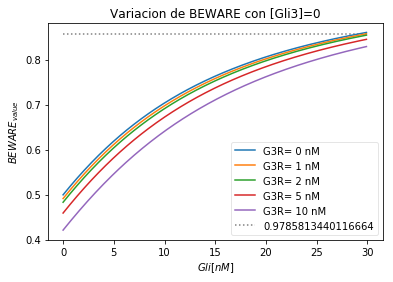
\includegraphics[width=0.8\textwidth]{variacion_new_beware}
	\centering
	\caption{Variación del nuevo operador BEWARE }
	\label{vari_beware}
\end{figure}

\begin{figure}[h]
	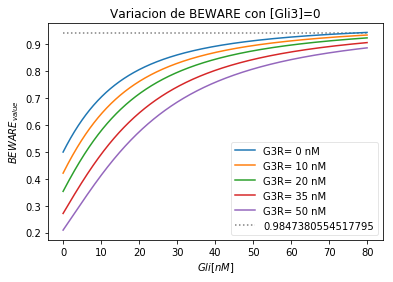
\includegraphics[width=0.8\textwidth]{variacion_new_beware_2}
	\centering
	\caption{Variación del nuevo operador BEWARE en más rango}
	\label{vari_beware_2}
\end{figure}

\subsection{Evolución temporal}

\begin{figure}[h]
	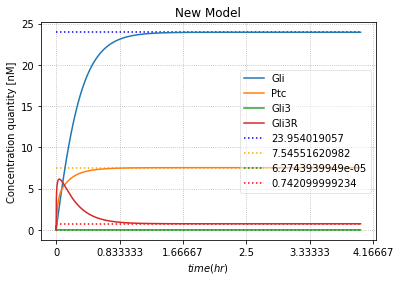
\includegraphics[width=0.8\textwidth]{new_beware_global}
	\centering
	\caption{Evolución temporal del nuevo operador BEWARE}
	\label{evolu_beware}
\end{figure}

\subsection{Análisis numérico de los estados estacionarios}


